% 	Name		:: 	sthlm Beamer Theme  HEAVILY based on the hsrmbeamer theme (Benjamin Weiss)
%	Author		:: 	Mark Hendry Olson (mark@hendryolson.com)
%	Created		::	2013-07-31
%	Updated		::	June 18, 2015 at 08:45
%	Version		:: 	1.0.2
%	Email		:: 	mark@hendryolson.com
%	Website		:: 	http://hendryolson.com
%
% 	License		:: 	This file may be distributed and/or modified under the
%                  	GNU Public License.
%
%	Description	::	This presentation is a demonstration of the sthlm beamer
%					theme, which is HEAVILY based on the HSRM beamer theme created by Benjamin Weiss
%					(benjamin.weiss@student.hs-rm.de), which can be found on GitHub
%					<https://github.com/hsrmbeamertheme/hsrmbeamert
%-=-=-=-=-=-=-=-=-=-=-=-=-=-=-=-=-=-=-=-=-=-=-=-=
%
%        LOADING DOCUMENT
%
%-=-=-=-=-=-=-=-=-=-=-=-=-=-=-=-=-=-=-=-=-=-=-=-=
%nosectionpage
\documentclass[newPxFont,sthlmFooter,nionpage]{beamer}
\usetheme{sthlm}

%-=-=-=-=-=-=-=-=-=-=-=-=-=-=-=-=-=-=-=-=-=-=-=-=
%        LOADING PACKAGES
%-=-=-=-=-=-=-=-=-=-=-=-=-=-=-=-=-=-=-=-=-=-=-=-=
\usepackage[utf8]{inputenc}

\usepackage{chronology}
\usepackage{algpseudocode}
\usepackage[Algorithmus]{algorithm}
\usepackage{xpatch}
\usepackage{pifont} %special symbols
\usepackage[utf8]{inputenc}
\usepackage{multirow}
\usepackage{tikz}
\usepackage{tkz-berge}
\usepackage{ulem}
\usetikzlibrary{shapes,snakes}

\xpatchcmd{\algorithmic}{\setcounter}{\algorithmicfont\setcounter}{}{}
\providecommand{\algorithmicfont}{}
\providecommand{\setalgorithmicfont}[1]{\renewcommand{\algorithmicfont}{#1}}
\renewcommand{\algorithmiccomment}[1]{{\tiny\hfill$\triangleright$ #1}}


\usepackage{changepage}

\renewcommand{\event}[3][e]{%
  \pgfmathsetlength\xstop{(#2-\theyearstart)*\unit}%
  \ifx #1e%
    \draw[fill=black,draw=none,opacity=0.5]%
      (\xstop, 0) circle (.2\unit)%
      node[opacity=1,rotate=45,right=.2\unit] {#3};%
  \else%
    \pgfmathsetlength\xstart{(#1-\theyearstart)*\unit}%
    \draw[fill=black,draw=none,opacity=0.5,rounded corners=.1\unit]%
      (\xstart,-.1\unit) rectangle%
      node[opacity=1,rotate=45,right=.2\unit] {#3} (\xstop,.1\unit);%
  \fi}%
%-=-=-=-=-=-=-=-=-=-=-=-=-=-=-=-=-=-=-=-=-=-=-=-=
%        BEAMER OPTIONS
%-=-=-=-=-=-=-=-=-=-=-=-=-=-=-=-=-=-=-=-=-=-=-=-=

%\setbeameroption{show notes}

\newtheorem{teo}{Teorema}
\numberwithin{teo}{section} 

% con * le indicamos que no lo debe numerar
\newtheorem{cor}{Corolario}
\numberwithin{cor}{section}


\newtheorem{pro}{Preguntas adicionales}
\numberwithin{pro}{section} 

\setbeamertemplate{caption}{\raggedright\insertcaption\par}

%-=-=-=-=-=-=-=-=-=-=-=-=-=-=-=-=-=-=-=-=-=-=-=-=
%
%	PRESENTATION INFORMATION
%
%-=-=-=-=-=-=-=-=-=-=-=-=-=-=-=-=-=-=-=-=-=-=-=-=
\title{Evaluation of Cayley Graphs}
\subtitle{for Parallel Computer Systems}
\date{International Conference on Computer, Information and Telecommunication Systems\\ \texttt{\small{\textcolor{black!80}{July 11-13, 2018 - Colmar, France}}}}
\author{\texttt{Daniela Aguirre Guerrero, Andreu Ma\~nosa, Llu\'is F\`abrega and Pere Vil\`a }}
\institute{
Universitat de Girona\\
}


\hypersetup{
pdfauthor = {Daniela Aguirre Guerrero: daniela.aguirre@udg.edu},
pdfsubject = {},
pdfkeywords = {},
pdfmoddate= {D:\pdfdate},
pdfcreator = {}
}

\begin{document}

%-=-=-=-=-=-=-=-=-=-=-=-=-=-=-=-=-=-=-=-=-=-=-=-=
%
%	TITLE PAGE
%
%-=-=-=-=-=-=-=-=-=-=-=-=-=-=-=-=-=-=-=-=-=-=-=-=

\maketitle

%\begin{frame}[plain]
%	\titlepage
%\end{frame}

%-=-=-=-=-=-=-=-=-=-=-=-=-=-=-=-=-=-=-=-=-=-=-=-=
%
%	TABLE OF CONTENTS: OVERVIEW
%
%-=-=-=-=-=-=-=-=-=-=-=-=-=-=-=-=-=-=-=-=-=-=-=-=
\begin{frame}[plain]{Agenda}
    \tableofcontents
\end{frame}


%-=-=-=-=-=-=-=-=-=-=-=-=-=-=-=-=-=-=-=-=-=-=-=-=
%
% SECTIONS
%
%-=-=-=-=-=-=-=-=-=-=-=-=-=-=-=-=-=-=-=-=-=-=-=-=
\section{Introduction}
% =================== CG properties =================== %
\subsection{Objective}
\begin{frame}[t]{Objective}
\begin{itemize}
    \item Evaluate the impact of \textbf{graph symmetry} on the \textbf{performance} and \textbf{robustness} of parallel computer systems.
    \item Aspects to evaluated:
    \begin{itemize}
        \item Connectivity
        \item Fault-tolerance
        \item Load balancing
    \end{itemize}
    \item Evaluated topologies:
    \begin{itemize}
        \item 3 symmetric Cayley Graphs (CG)
        \item 2 non-symmetric CG
        \item 3 Data Center Networks (DCN)
    \end{itemize}
\end{itemize}
\end{frame}
% =================== CG =================== %
\subsection{Cayley Graphs}
\begin{frame}[t]{Cayley Graphs}
\begin{itemize}
    \item A CG is a geometric representation of an algebraic group.
    \item CGs have regular degree ($\Delta$) and grow increasing their degree.
\end{itemize}
\scriptsize
\begin{table}[]
\centering{
\begin{tabular}[center]{c c c}
\includegraphics{images/tikz/square.tikz}
&\includegraphics{images/tikz/cube.tikz}
&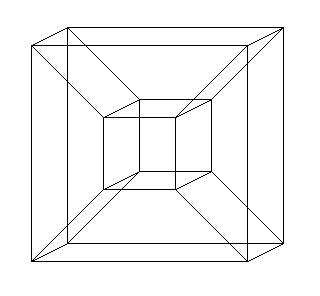
\includegraphics[width=0.245\textwidth]{images/cube4}
\\
\textbf{$\Delta=2$}&\textbf{$\Delta=3$}&\textbf{$\Delta=4$}\\
\end{tabular}
\caption{Family of Hypercube graphs}
}
\end{table}
\end{frame}
% =================== CG properties =================== %
%\begin{frame}[t]{Cayley Graphs: Properties}
%\begin{itemize}
%    \item Recursive graphs.
%    \item Node-transitive.
%    \item Some CGs have constant degree or constant diameter.
%\end{itemize}
%\scriptsize
%\begin{table}[]
%\centering{
%\begin{tabular}[center]{c c c}
%\includegraphics{images/tikz/square.tikz}
%&\includegraphics{images/tikz/cube.tikz}
%&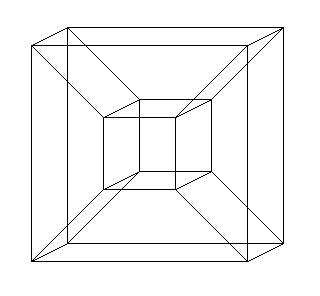
\includegraphics[width=0.245\textwidth]{images/cube4}
%\\
%\textbf{$\Delta=2$}&\textbf{$\Delta=3$}&\textbf{$\Delta=4$}\\
%\end{tabular}
%\caption{Family of Hypercube graphs}
%}
%\end{table}
%\end{frame}
%========================================= %
\begin{frame}{Cayley graphs as Model of Interconnection Networks}
\begin{itemize}
\item Processor Interconnection Networks (PIN) [1-2].
\item Data Center Networks (DCN) [3-4].
\end{itemize}
\center{
    \begin{tabular}{c c c}
        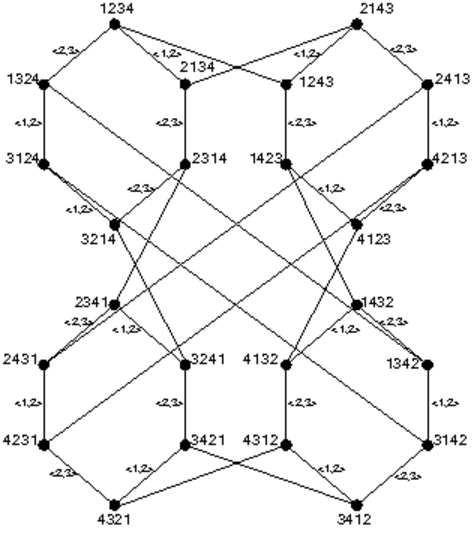
\includegraphics[width=0.25\textwidth]{images/nets/bubble_sort.pdf}
        %& 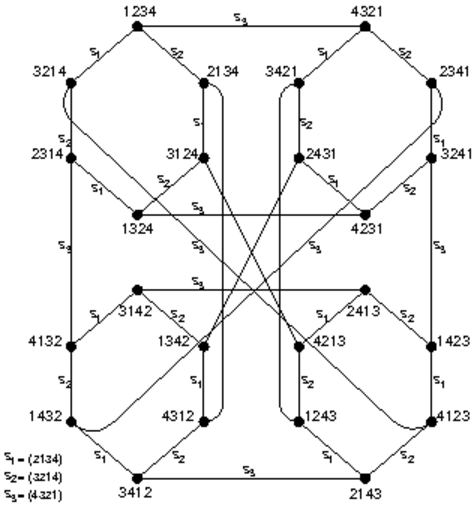
\includegraphics[width=0.3\textwidth]{images/nets/pancake.pdf}
        &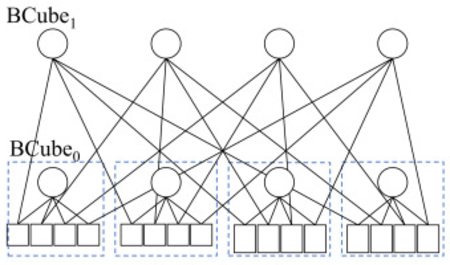
\includegraphics[width=0.5\textwidth]{images/nets/bcube.pdf}\\
        \textbf{\footnotesize Star}
        %& \textbf{\footnotesize Pancake}
        & \textbf{\footnotesize Bcube}\\
    \end{tabular}    }
\flushleft{\tiny
\begin{enumerate}[{[1]}]
	\item M. Heydemann, "Cayley graphs and interconnection networks," on NATO ASI Series: Mathematical and Physical Sciences, vol 497. Springer, 1997. 
    \item T. Stephen et. all, "Processor interconnection networks from Cayley graphs," in Discrete Applied Mathematics, vol. 40, 1992. 
    \item Ch. Guo et. all, "BCube: a high performance, server-centric network architecture for modular data centers,"  in Proc. of the ACM-SIGCOMM, 2009. 
    \item J. Kim et. all, "Flattened butterfly: a cost-efficient topology for high-radix networks,"  in Proc. of the ISCA, 2007. 
    %\item B. Andruset. all, "SDN data center performance evaluation of torus and hypercube interconnecting schemes,"  in Proc. of the RTUWO, 2015.
\end{enumerate}}
\end{frame} 
%========================================= %
%\begin{frame}{Cayley graphs as Models of Interconnection Networks (2/2)}
%\begin{itemize}
%\item Data Center Networks (DCN)\end{itemize}
%\center{
%    \begin{tabular}{c c c}
%        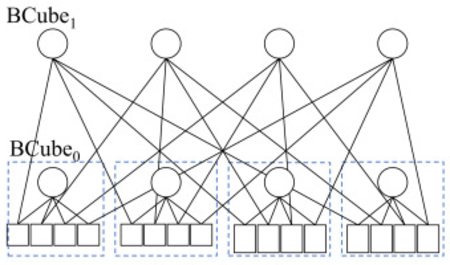
\includegraphics[width=0.28\textwidth]{images/nets/bcube.pdf}& 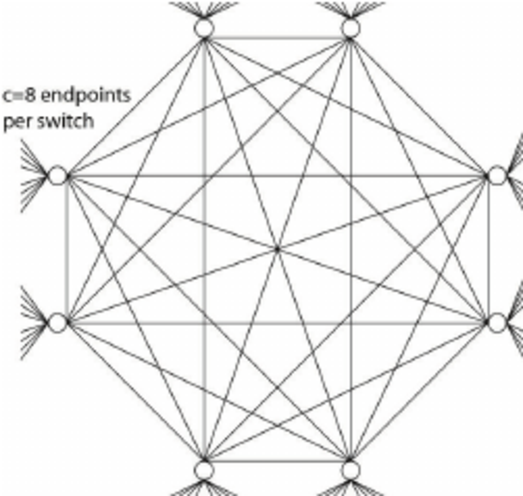
\includegraphics[width=0.21\textwidth]{images/nets/butterfly.pdf}&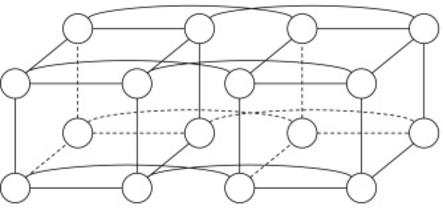
\includegraphics[width=0.28\textwidth]{images/nets/hypercube.pdf}\\
%        \textbf{\footnotesize BCube [3]}& \textbf{\footnotesize Flattened Butterfly [4]}& \textbf{\footnotesize Hypercube [5]}\\
%    \end{tabular}  }
%\flushleft{\tiny
%\begin{enumerate}[{[1]}]
%    \setcounter{enumi}{2}
%	\item Ch. Guo et. all, "BCube: a high performance, server-centric network architecture for modular data centers,"  in Proc. of the ACM-SIGCOMM, 2009. 
%    \item J. Kim et. all, "Flattened butterfly: a cost-efficient topology for high-radix networks,"  in Proc. of the ISCA, 2007. 
%    \item B. Andruset. all, "SDN data center performance evaluation of torus and hypercube interconnecting schemes,"  in Proc. of the RTUWO, 2015.
%\end{enumerate}}
%\end{frame}
\subsection{Symmetry}
% =================== Symmetry =================== %
\begin{frame}[t]{Symmetry Measures}
\begin{enumerate}
\item \textbf{Node-transitivity}. All the nodes have the same \textit{perspective} of the whole network graph. 

CGs are node-transitive.
\item \textbf{Link-transitivity}. All the links have the same \textit{perspective} of the whole network graph. 

Some CGs are link-transitive
\end{enumerate}
\scriptsize
\centering{
\begin{tabular}[center]{c c c c}
\includegraphics{images/tikz/triangle.tikz}
&\includegraphics{images/tikz/3path.tikz}
&\includegraphics{images/tikz/cube.tikz}
&\includegraphics{images/tikz/any_graph.tikz}
\\
\textbf{node-transitive}&\textbf{link-transitive}&\textbf{node and link-transitive}&\textbf{non-transitive}\\
&&\textbf{(symmetric graph)}
\end{tabular}
}
\end{frame}

\section{Evaluation of Topologies}
\subsection{Connectivity and Fault-tolerance}
% =================== Connectivity =================== %
\begin{frame}[t]{Connectivity Measures}
\begin{enumerate}
\item \textbf{Node connectivity} ($c_n$). 
\begin{itemize}
\item \textbf{Minimal number of node-disjoint} paths between any pair of nodes.
\item \textbf{Minimal number of nodes} that must be removed to disconnect the network.
\end{itemize}
\item \textbf{Link connectivity} ($c_l$). 
\begin{itemize}
\item \textbf{Minimal number of link-disjoint} paths between any pair of nodes.
\item \textbf{Minimal number of links} that must be removed to disconnect the network.
\end{itemize}
\end{enumerate}
\end{frame}
% =================== Optimal Connectivity =================== %
\begin{frame}[t]{Optimal Connectivity}

\begin{itemize}
\item A $\Delta-$regular graph is \textbf{optimally connected} if $c_n=c_l=\Delta$.
\item Every \textbf{node-transitive} graph has $c_n=\Delta$.
\item Every \textbf{link-transitive} graph has $c_l=\Delta$.
\end{itemize}
\centering{
\begin{tabular}[center]{c c}
\includegraphics<1>{images/tikz/scaleCube1.tikz}
\includegraphics<2>{images/tikz/scaleCube2.tikz}
\includegraphics<3>{images/tikz/scaleCube3.tikz}
\includegraphics<4>{images/tikz/scaleCube4.tikz}
\includegraphics<5>{images/tikz/scaleCube5.tikz}
\includegraphics<6>{images/tikz/scaleCube6.tikz}
\includegraphics<7-10>{images/tikz/scaleCube2.tikz}
&\includegraphics<1-6>{images/tikz/3regular1.tikz}
\includegraphics<7>{images/tikz/3regular2.tikz}
\includegraphics<8>{images/tikz/3regular3.tikz}
\includegraphics<9>{images/tikz/3regular4.tikz}
\includegraphics<10>{images/tikz/3regular5.tikz}
\\
\textbf{Optimally connected}&\textbf{Non-optimally connected}\\
$c_n=c_l=\Delta=3$&$c_n=c_l=2$\\
\end{tabular}
}
\end{frame}
% =================== Fault-tolerance =================== %
\begin{frame}[t]{Fault-tolerance}
\begin{itemize}
\item Maximal number $f$, such that if $f$ nodes are removed, the resulting graph is still connected.
\item A $\Delta$-regular graph is \textbf{optimally fault-tolerant} if $f=\Delta-1$.
\item \textbf{Symmetric graphs} are optimally fault-tolerant.
\end{itemize}
\centering{
\begin{tabular}[center]{c c}
\includegraphics<1>{images/fault_tolerance/scaleCube1.tikz}
\includegraphics<2>{images/fault_tolerance/scaleCube2.tikz}
&\includegraphics<1>{images/fault_tolerance/3regular1.tikz}
\includegraphics<2>{images/fault_tolerance/3regular2.tikz}
\\
\textbf{Optimally fault-tolerant}&\textbf{Non-optimally fault-tolerant}\\
$f=\Delta-1=2$&$f=1$\\
\end{tabular}
}
\end{frame}
% =================== Connectivity and fault-tolerance =================== %
%\begin{frame}[t]{Connectivity and Fault-tolerance}
%\begin{table}
    \begin{tabular}{l c c c}
      \toprule
      \multirow{2}{*}{\textbf{Cayley graph}}&\multirow{2}{*}{\textbf{Symmetric}}&\textbf{Optimally}&\textbf{Optimally}\\
      &&\textbf{connected}&\textbf{fault-tolerant}\\
      \midrule
      Bubble-sort & \multirow{2}{*}{\centering{No}}&\multirow{2}{*}{\centering{No}}&\multirow{2}{*}{\centering{No}}\\
      Butterfly & \\
      \hline
      Star & \multirow{3}{*}{\centering{Yes}}& \multirow{3}{*}{\centering{Yes}}& \multirow{3}{*}{\centering{Yes}}\\
      Transposition & \\
      Hypercube & \\
      \bottomrule
    \end{tabular}
    \caption{Evaluated Cayley Graphs}
  \end{table}
  
%\end{frame}
\subsection{Moore Bound}
% =================== Deg-Diam problem =================== %
\begin{frame}[t]{Moore Bound: the Degree-diameter Problem}
\begin{itemize}
\item Connect the \textbf{maximum number of routers} ($n$) while keeping \textbf{small length of paths} ($D_{avg}$) and considering that \textbf{the number of router ports is limited} $(\Delta)$.
\item For any $\Delta$-regular graph
$$\displaystyle D\geq \frac{\log(n-1)}{\log(\Delta)}.$$
\item For any node-transitive graph 
$$\displaystyle D_{avg}\geq \frac{nD}{2(n-1)}.$$
\end{itemize}
\end{frame}
% =================== Moore bound =================== %
%\begin{frame}[t]{Moore Bound: Diameter}
%\begin{itemize}
%\item For any $\Delta$-regular graph
% $\displaystyle D\geq \frac{\log(n-1)}{\log(\Delta)}$.
%\end{itemize}
%\begin{table}[h!]
    \begin{tabular}{|c| l |c|}
      \toprule
      \multicolumn{2}{|c|}{\textbf{Topology}}&\multirow{1}{*}{\textbf{$D$}}\\
      \midrule
      \multirow{3}{*}{\textbf{DCN}}&Slimfly & 2\\
      &Jellyfish & 3\\
      &Fat-tree &4\\
      \hline
      \multirow{2}{*}{\textbf{Symmetric}}&Star &\multirow{3}{*}{$O(\log(n))$}\\
      \multirow{2}{*}{\textbf{CG}}&Transposition & \\
      &Hypercube& \\
      \hline
      \multirow{1}{*}{\textbf{Non-symmetric}}&Butterfly&\multirow{1}{*}{$O(\log(n))$}\\
      \multirow{1}{*}{\textbf{CG}}&Bubble-sort& $O(\log(n)^2)$\\
      \bottomrule
    \end{tabular}
  \end{table}
%\end{frame}

% =================== Moore bound =================== %
\begin{frame}[t]{Moore bound: Average Path Distance}
%\begin{itemize}
%\item For any node-transitive graph 
%$\displaystyle D_{avg}\geq \frac{nD}{2(n-1)}$.
%\end{itemize}
\center{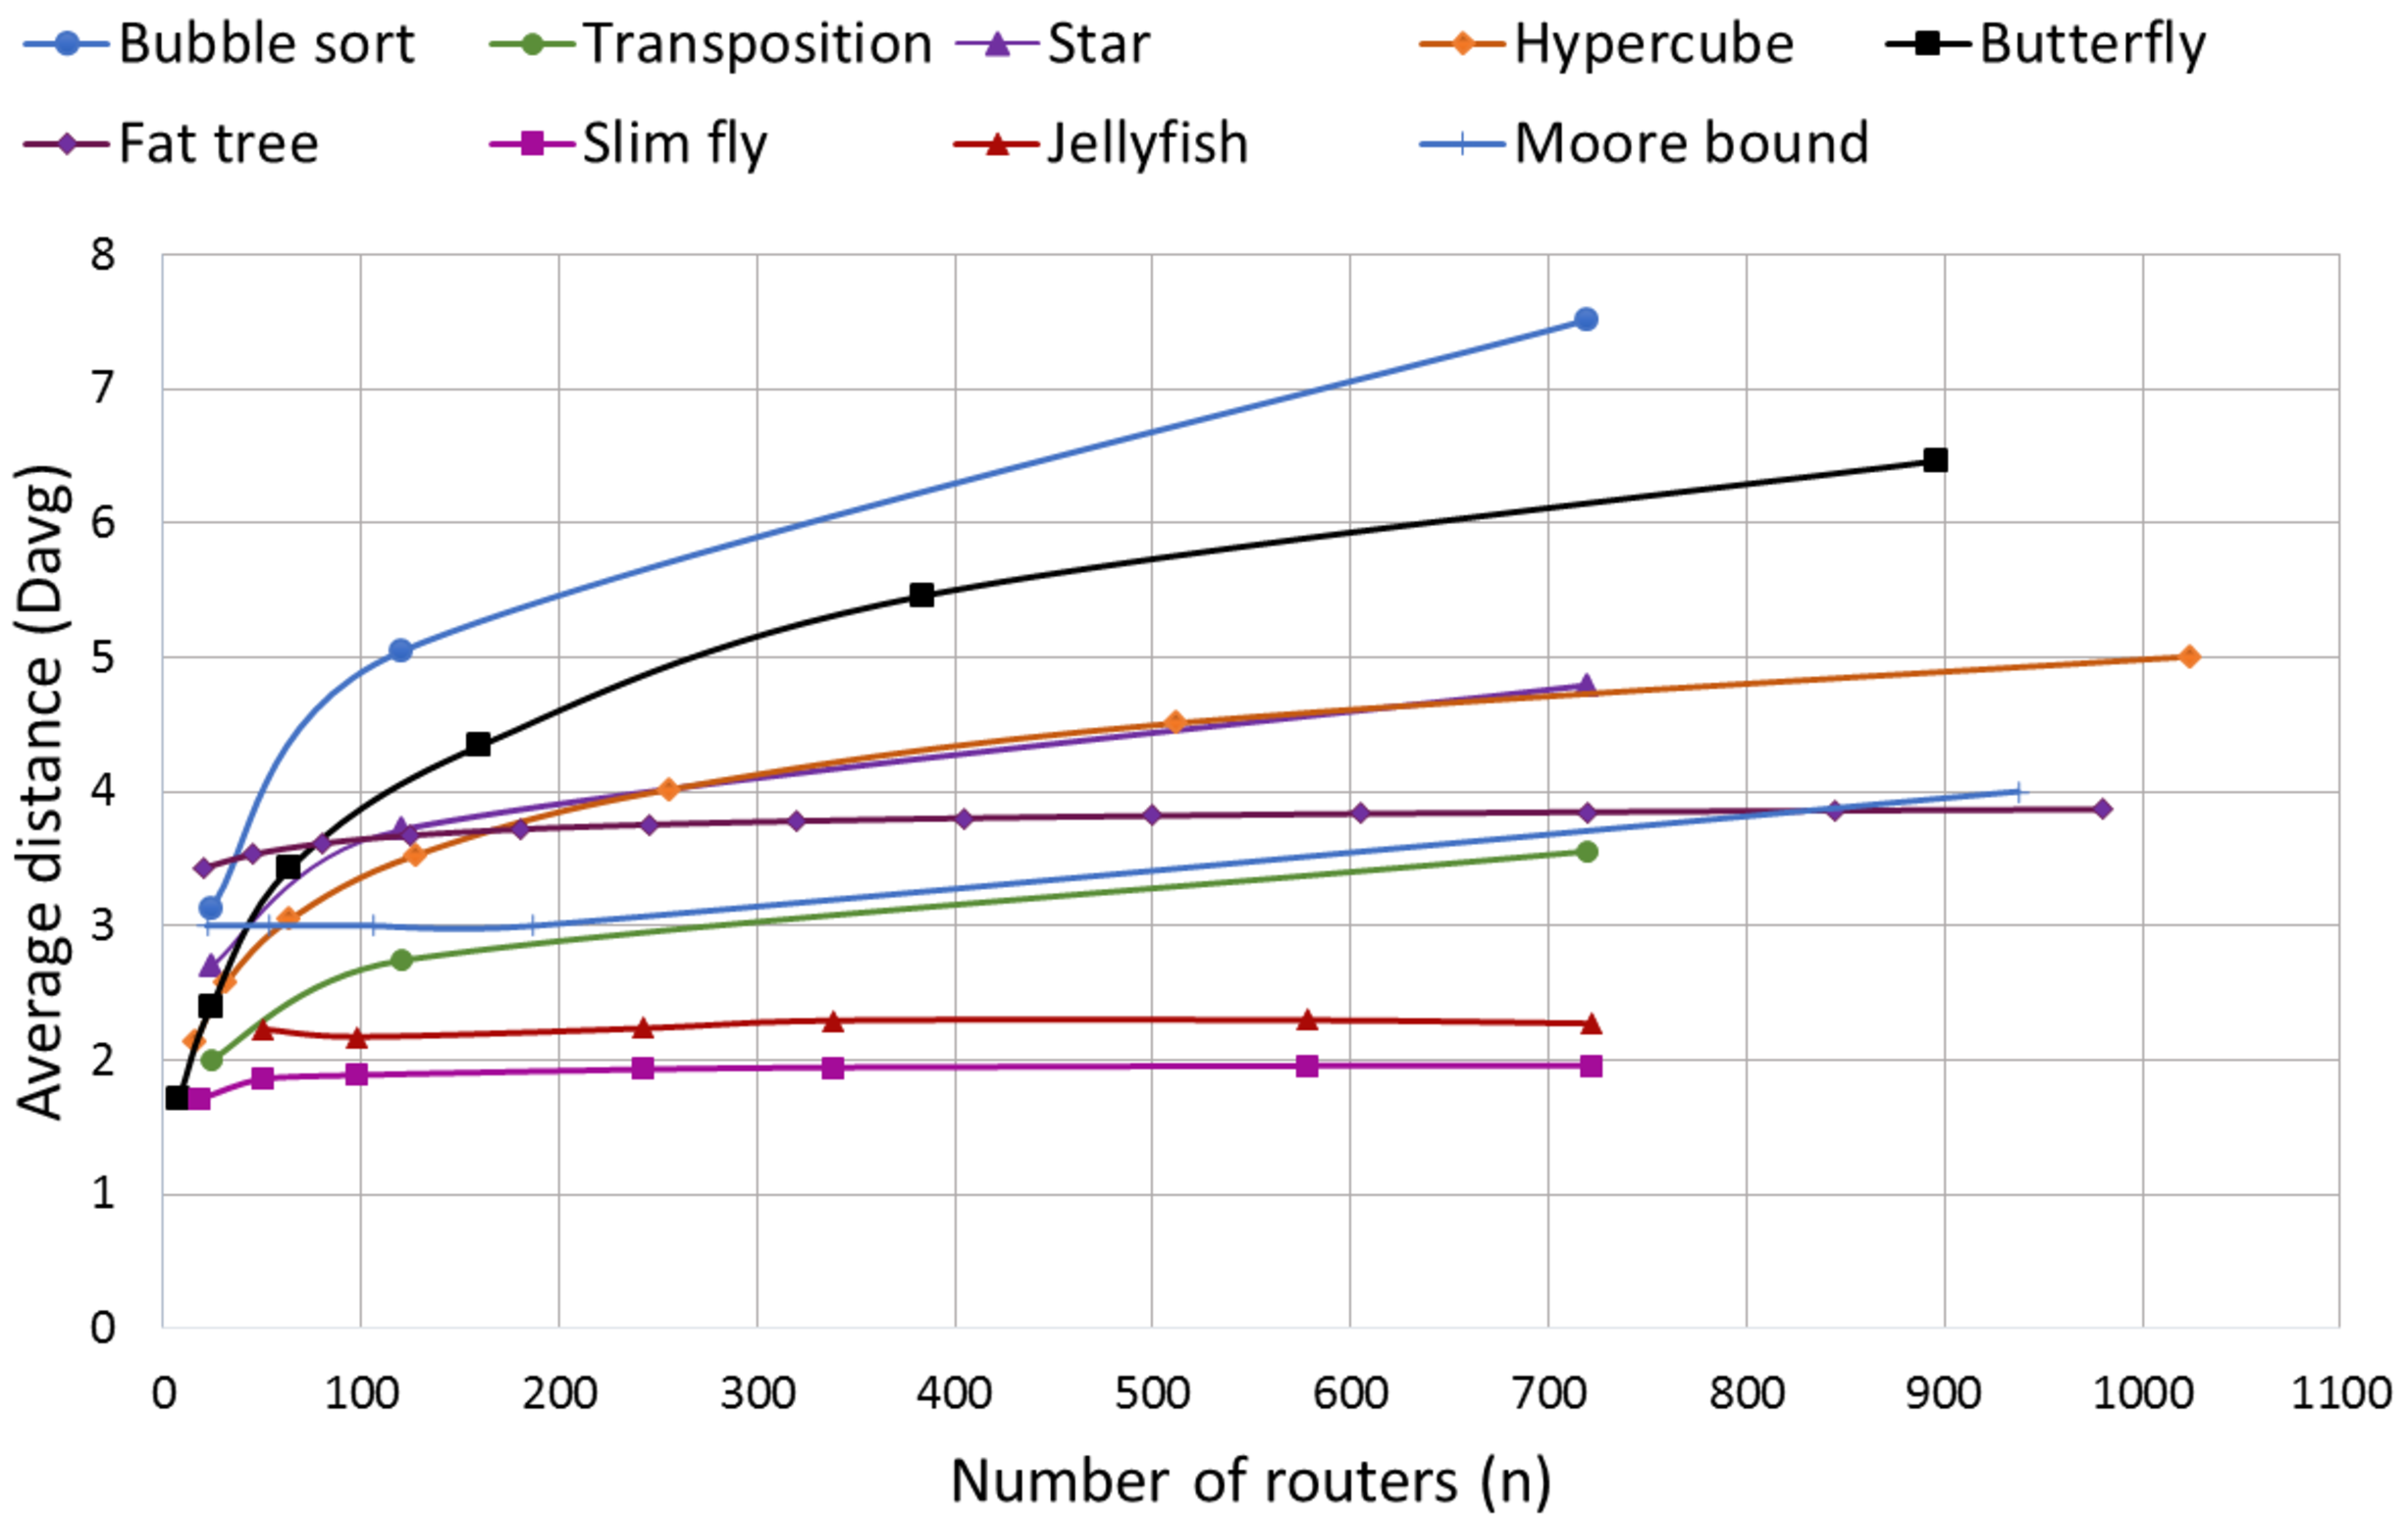
\includegraphics[width=.95\textwidth]{images/avgdist}}
\end{frame}
\subsection{Load Balancing}
% =================== Assumptions =================== %
\begin{frame}[t]{Load Balancing: Link Load}

\begin{itemize}
\item Assumptions:

\begin{itemize}
\item Uniform traffic pattern.
\item Ideal routing.
\end{itemize}
\item The \textbf{load of a link} $e$, i.e. $l_{e}$, is the amount of traffic units traversing $e$ per cycle.
\item The \textbf{average link load} is $\displaystyle l_{avg}=\frac{\sum{l_e}}{\#\textnormal{ links}}$.
\item A network reaches the \textbf{saturation point} when \textbf{some link has the maximum link load} ($l_{max}= \max\{l_e\}$).
\end{itemize}
\end{frame}
% =================== Link load =================== %
\begin{frame}[t]{Load Balancing: Average Link Utilization }
\begin{itemize}
\item The average link utilization at the saturation point ($u_{avg}$) is
$$\displaystyle u_{avg}=\frac{l_{avg}}{l_{max}}.$$
\item \textbf{Symmetric graphs} are well-balanced, i.e. $u_{avg}=1$.
\end{itemize}
%\center{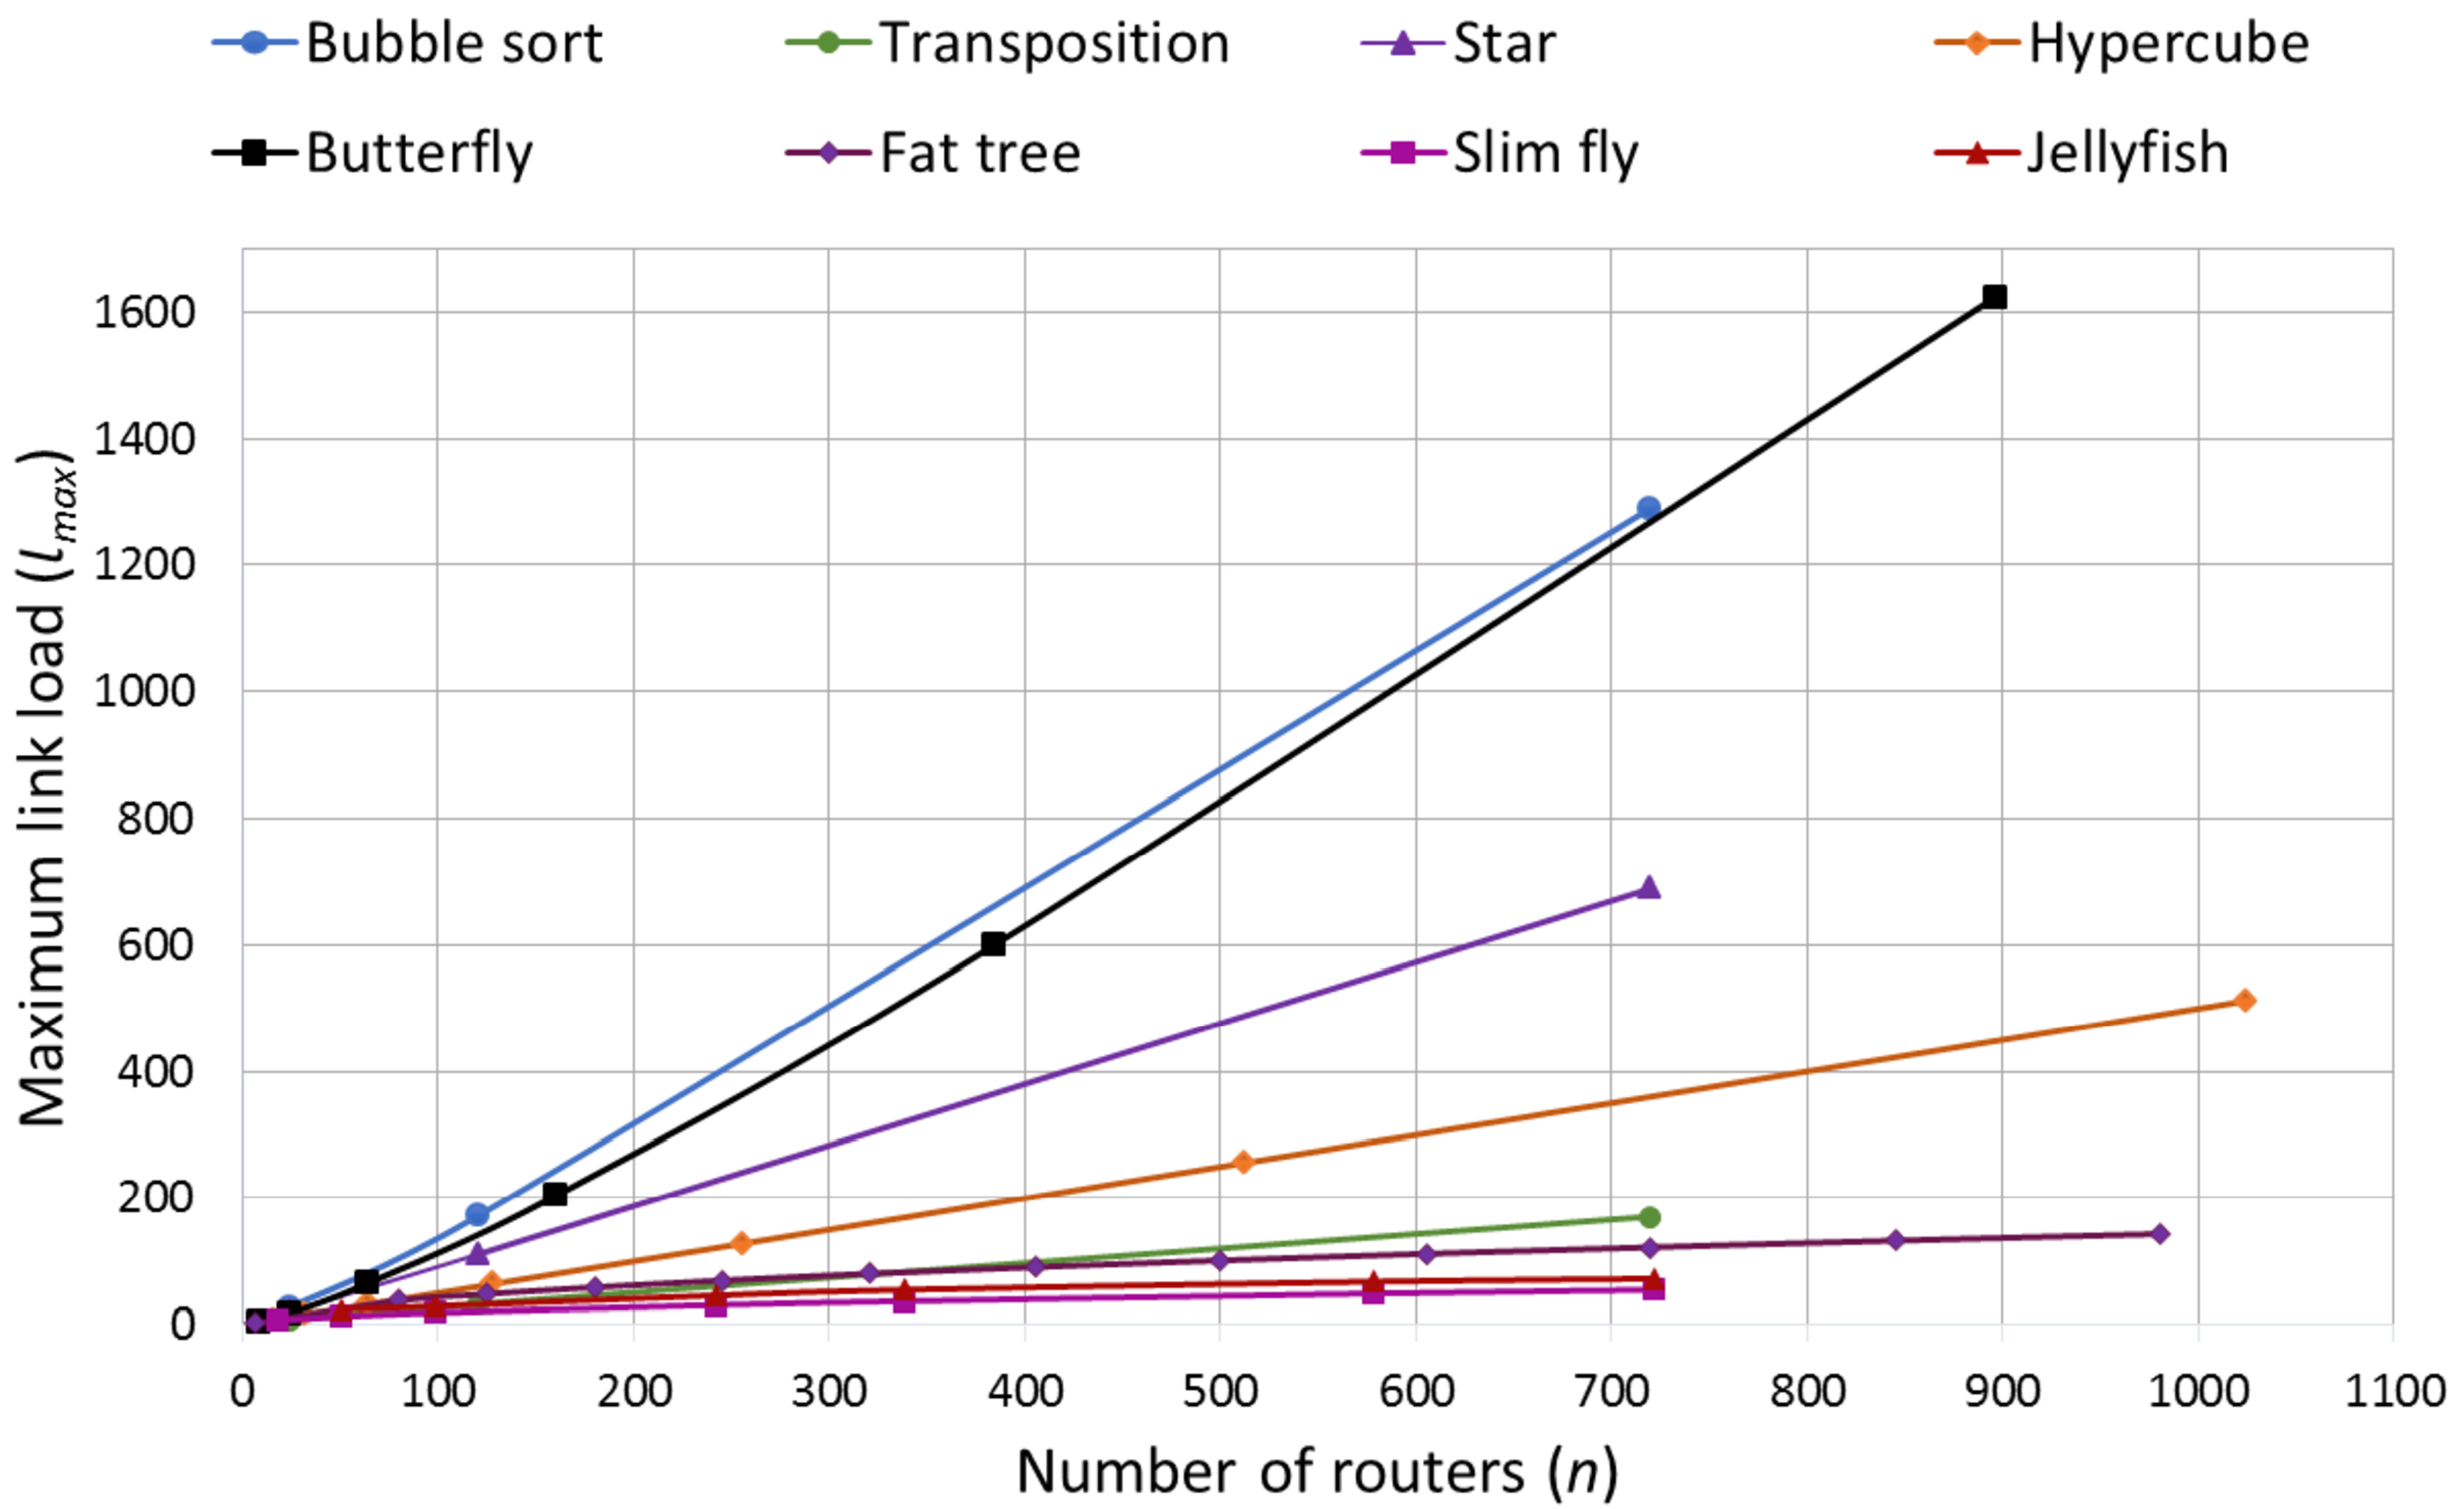
\includegraphics[width=0.85\textwidth]{images/maxll}}
\end{frame}

% =================== Link load =================== %
%\begin{frame}[t]{Load Balancing: Well-balanced Networks}
%\footnotesize
\begin{table}[h!]
    \begin{tabular}{|c| l |c|c|}
      \toprule
      \multicolumn{2}{|c|}{\multirow{2}{*}{\textbf{Topology}}}&\multirow{1}{*}{\textbf{Moore}}&\multirow{1}{*}{\textbf{Symmetric}}\\
      \multicolumn{2}{|c|}{}&\multirow{1}{*}{\textbf{Graph}}&\multirow{2}{*}{}\\
      \midrule
      \multirow{3}{*}{\textbf{DCN}}&Slimfly & \multirow{3}{*}{No}& \multirow{3}{*}{No}\\
      &Jellyfish & \\
      &Fat-tree &\\
      \hline
      \multirow{2}{*}{\textbf{Symmetric}}&Star & \multirow{3}{*}{No}&\multirow{3}{*}{Yes}\\
      \multirow{2}{*}{\textbf{CG}}&Transposition & \\
      &Hypercube& \\
      \hline
      \multirow{1}{*}{\textbf{Non-symmetric}}&Butterfly&\multirow{2}{*}{No}\\
      \multirow{1}{*}{\textbf{CG}}&Bubble-sort& \\
      \bottomrule
    \end{tabular}
  \end{table}
%\end{frame}
% =================== Link load =================== %
\begin{frame}[t]{Load Balancing: Amount of Workstations Supported}
\begin{itemize}
\item \textbf{Maximum number of end points} $\Delta_p$ supported by each router \textbf{without reaching the saturation point}.
$$\displaystyle\Delta_p\leq \frac{\Delta u_{avg}}{D_{avg}}$$
\end{itemize}
\end{frame}
% ================ End points - n ================ %
\begin{frame}[t]{Amount of Workstations with Respect to the Network Size}
\center{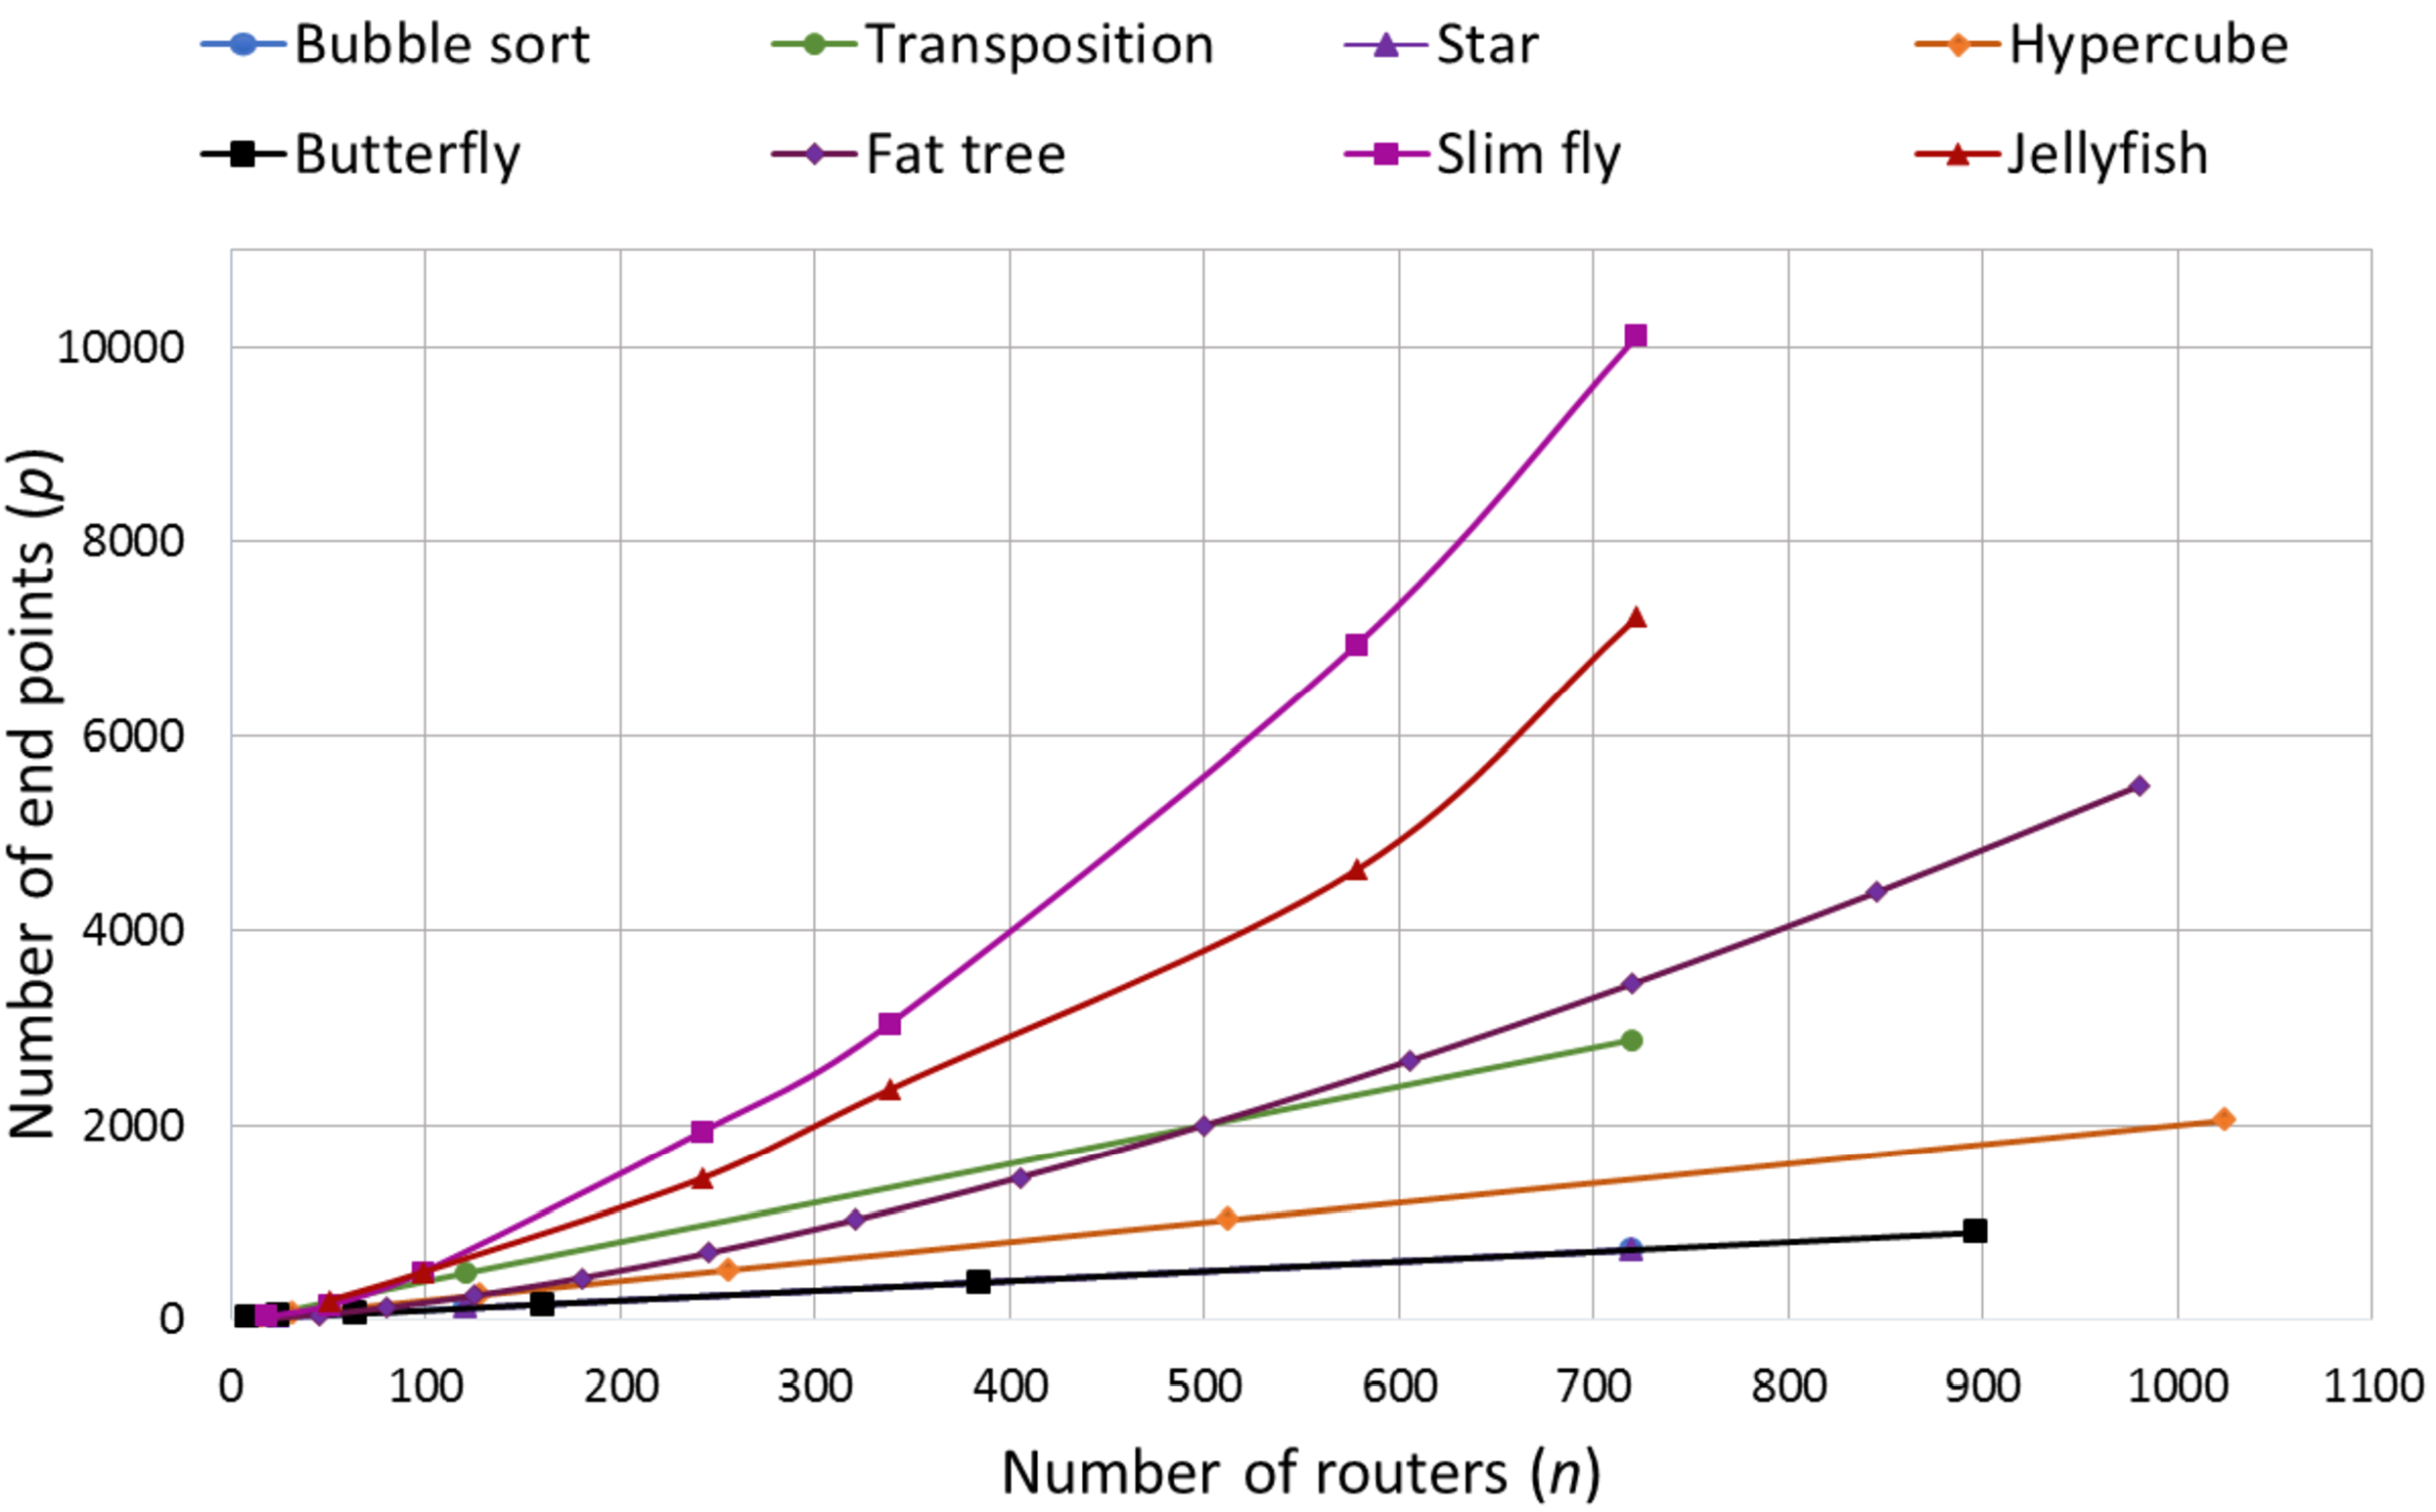
\includegraphics[width=\textwidth]{images/enpXserv}}
\end{frame}
% ================ End points - radix ================ %
\begin{frame}[t]{Amount of Workstations with Respect to the Router Radix}
\center{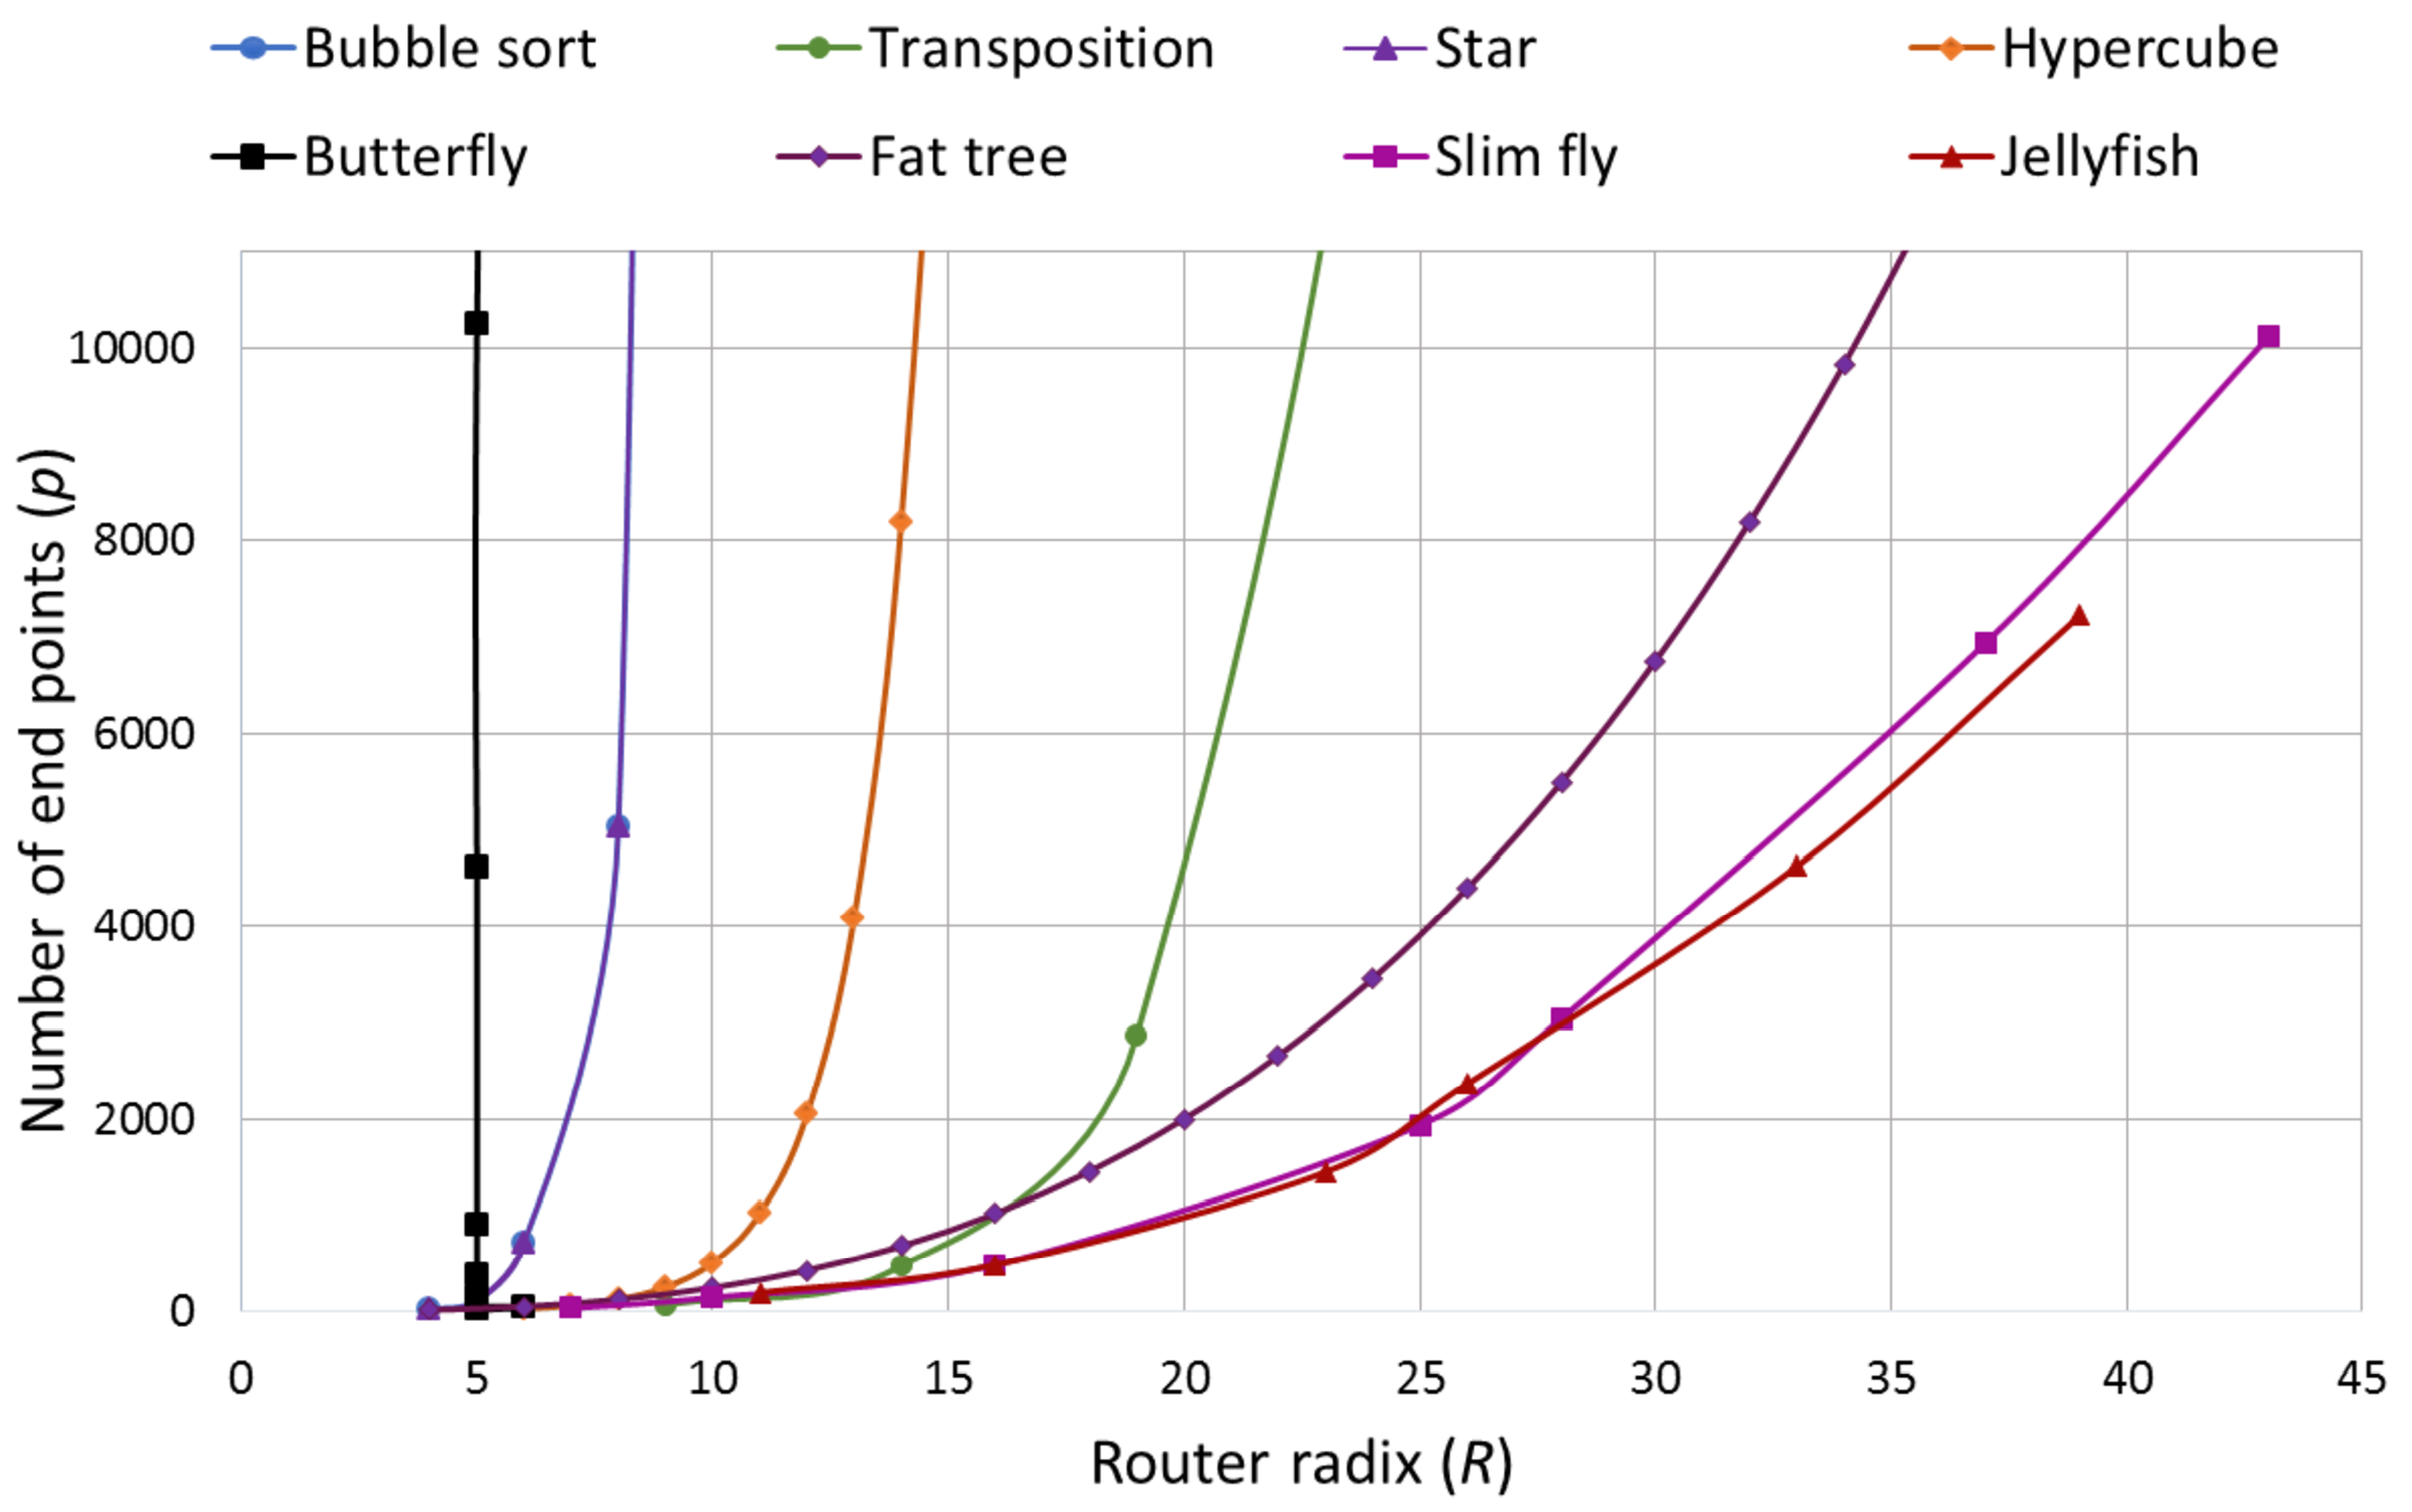
\includegraphics[width=\textwidth]{images/enpXradix}}
\end{frame}
% =================== Link load =================== %
\begin{frame}[t]{Load Balancing: Average Link Utilization ($u_{avg}$)}
\begin{itemize}
\item Percentage of link utilization at the saturation point.%, i.e.
%$$\displaystyle u_{avg}=\frac{l_{avg}}{l_{max}}.$$
%\item A network is \textbf{well-balanced} if $\displaystyle u_{avg}=1$.
\end{itemize}
\footnotesize
\begin{table}[h!]
    \begin{tabular}{|c| l |c|c|}
      \toprule
      \multicolumn{2}{|c|}{\multirow{2}{*}{\textbf{Topology}}}&\multirow{1}{*}{\textbf{Moore}}&\multirow{1}{*}{\textbf{Symmetric}}\\
      \multicolumn{2}{|c|}{}&\multirow{1}{*}{\textbf{Graph}}&\multirow{2}{*}{}\\
      \midrule
      \multirow{3}{*}{\textbf{DCN}}&Slimfly & \multirow{3}{*}{No}& \multirow{3}{*}{No}\\
      &Jellyfish & \\
      &Fat-tree &\\
      \hline
      \multirow{2}{*}{\textbf{Symmetric}}&Star & \multirow{3}{*}{No}&\multirow{3}{*}{Yes}\\
      \multirow{2}{*}{\textbf{CG}}&Transposition & \\
      &Hypercube& \\
      \hline
      \multirow{1}{*}{\textbf{Non-symmetric}}&Butterfly&\multirow{2}{*}{No}\\
      \multirow{1}{*}{\textbf{CG}}&Bubble-sort& \\
      \bottomrule
    \end{tabular}
  \end{table}
\end{frame}
% ================ Symmetric Properties ================ %
%\begin{frame}[t]{Evaluation of Networks with about 1000 Routers}
%\small
\centering
\begin{tabular}[center]{|c|c|c|c|c|c|}
\toprule
\multicolumn{2}{|c|}{\multirow{2}{*}{\textbf{Topology}}}&\multirow{2}{*}{$n$}&\multirow{2}{*}{$D_{avg}$}&\multirow{2}{*}{$u_{avg}$}&\multirow{2}{*}{$\Delta_p$}\\
\multicolumn{2}{|c|}{}&&&&\\
\midrule
\multirow{3}{*}{\textbf{DCN}}&\multirow{1}{*}{Slimfly} &\multirow{1}{*}{722}&\multirow{1}{*}{1.96}&\multirow{1}{*}{0.95}&\multirow{1}{*}{15}\\
%& & &&\\
%\hline
&\multirow{1}{*}{Jellyfish} &\multirow{1}{*}{722}&\multirow{1}{*}{2.27}&\multirow{1}{*}{0.82}&\multirow{1}{*}{15}\\
%& & &&\\
%\hline
&\multirow{1}{*}{Fat-tree} &\multirow{1}{*}{720}&\multirow{1}{*}{3.09}&\multirow{1}{*}{0.99}&\multirow{1}{*}{12}\\
%& & &&\\
\hline
\multirow{2}{*}{\textbf{Symmetric}}&\multirow{1}{*}{Transposition} &\multirow{1}{*}{720}&\multirow{1}{*}{3.55}&\multirow{1}{*}{1}&\multirow{1}{*}{4}\\
%& & &&\\
%\hline
\multirow{2}{*}{\textbf{CG}}&\multirow{1}{*}{Hypercube} &\multirow{1}{*}{1024}&\multirow{1}{*}{5}&\multirow{1}{*}{1}&\multirow{1}{*}{2}\\
%& & &&\\
%\hline
&\multirow{1}{*}{Star} &\multirow{1}{*}{720}&\multirow{1}{*}{4.79}&\multirow{1}{*}{1}&\multirow{1}{*}{1}\\
%& & &&\\
\hline
\multirow{1}{*}{\textbf{Non-symmetric}}&\multirow{1}{*}{Bubble-sort} &\multirow{1}{*}{720}&\multirow{1}{*}{7.50}&\multirow{1}{*}{0.86}&\multirow{1}{*}{1}\\
%& & &&\\
%\hline
\multirow{1}{*}{\textbf{CG}}&\multirow{1}{*}{Butterfly} &\multirow{1}{*}{896}&\multirow{1}{*}{6.46}&\multirow{1}{*}{0.86}&\multirow{1}{*}{1}\\
%& & &&\\
\bottomrule
\end{tabular}
%\end{frame}
\section{Conclusions}
% =================== Conclusions =================== %
\begin{frame}[t]{Conclusions (1/2)}
\begin{itemize}
    \item Symmetric networks:
    \begin{itemize}
        \item allows the use of \textbf{simple communication protocols}.
        \item provide \textbf{optimal fault-tolerance} for random failures, and
        \item \textbf{balance traffic} equally across link.
    \end{itemize}
    \item Moore networks provide:
    \begin{itemize}
        \item \textbf{low latency}, and
        \item \textbf{low link load}, thereby supporting a \textbf{high number of workstations}.
    \end{itemize}     
    \item Modern DCN topologies have been designed according to the Moore bound. However, they are not symmetric.
    \item Some CGs have been used as model of PIN and DCN. However, most of them do not satisfy the Moore bound.
\end{itemize}
\end{frame}
% =================== Conclusions =================== %
\begin{frame}[t]{Conclusions (2/2)}
\begin{itemize}
    \item CGs provide a useful interconnection model for parallel computer systems that are symmetric and satisfy the Moore bound, e.g. Transposition graph.
    \item Some challenges:
    \begin{itemize}
        \item Design methods for incremental expansion in the number of routers.
        \item Design methods for reduce the diameter by increasing the number of links between routers.
    \end{itemize}
\end{itemize}
\end{frame}
\begin{frame}[plain,c]

\center{\Huge\textcolor{white}{.\\.\\.\\}\textmd{Questions...}\textcolor{white}{\\.\\.}}
\flushright{\scriptsize{\textcolor{gray}{Daniela Aguirre Guerrero\\daniela.aguirre@udg.edu\\ \url{https://daniaguirre.github.io}}}}
\end{frame}

%-=-=-=-=-=-=-=-=-=-=-=-=-=-=-=-=-=-=-=-=-=-=-=-=
%
% REFERENCES
%
%-=-=-=-=-=-=-=-=-=-=-=-=-=-=-=-=-=-=-=-=-=-=-=-=

%\section{References}
%\begin{frame}[allowframebreaks]{References}
%  \bibliography{Bibliografia}
%  \bibliographystyle{abbrv}
%\end{frame}

%\input{examples.tex}
\end{document}